\scanpage{28}
\mspage{\handwritten{\unsure{7|2}2}}
% archive sheet number: 27 (inverted at the upper right)
% Whole source: 1683 x 2140. The three outer deletion macros mark the page-wide cancellation.
% GRAPHIC G01: the actual long, slightly bowed cancellation stroke, source x=730--858, y=245--2115.
% Its shape is reproduced separately; the outer deletion macros identify the text crossed by it.
\handwritten{\figure{\begin{tikzpicture}[x=.004cm,y=-.004cm]
\draw[line width=.35pt] (847,245) .. controls (832,327) and (813,402) .. (817,485)
 .. controls (834,692) and (858,958) .. (857,1165)
 .. controls (855,1445) and (822,1685) .. (801,1842)
 .. controls (786,1951) and (756,2043) .. (730,2115);
\end{tikzpicture}}}

\deleted{un morphisme de topos $\mathrm{u}:\mathrm{E}\handwritten{\longrightarrow}\mathrm{E}'$, et ce dernier sera ``unique à isomorphisme unique près'' en termes de la donnée $\mathrm{u}^{\handwritten{*}}$ resp. $\mathrm{u}_{\handwritten{*}}$, en un sens assez clair, et qui sera d'ailleurs entièrement explicité plus bas \handwritten{(\deleted{\unsure{2|3}}3.2.1)}\unsure{.}}
% The final point is partially clipped at the right edge; its status as punctuation remains uncertain.

\deleted{\deleted{2}\handwritten{3}.1.2. Si $\mathrm{u}:\mathrm{E}\handwritten{\longrightarrow}\mathrm{E}'$ est un morphisme de topos, il résulte des propriétés des foncteurs adjoints
% GRAPHIC G02: raised reference and its curved leader before que.
\mbox{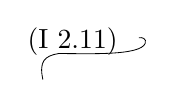
\begin{tikzpicture}[baseline=(b.base),x=1cm,y=1cm]
\node[anchor=base west,inner sep=0pt] (b) at (0,0) {\strut};
\node[anchor=south west,inner sep=0pt] at (-.2,.20) {\inserted{\handwritten{(I 2.11)}}};
\draw[line width=.3pt] (0,-.10) .. controls (-.05,.13) and (.02,.20) .. (.20,.23) .. controls (.58,.23) and (1.24,.20) .. (1.30,.36) .. controls (1.32,.42) and (1.26,.44) .. (1.22,.43);
\end{tikzpicture}}que le foncteur image directe $\mathrm{u}_{\handwritten{*}}:\mathrm{E}\handwritten{\longrightarrow}\mathrm{E}'$ commute aux limites projectives, et le foncteur $\mathrm{u}^{\handwritten{*}}:\mathrm{E}'\handwritten{\longrightarrow}\mathrm{E}$ commute aux limites inductives \deleted{\unsure{(2.11)|(2.1)|(I 2.11)}}\handwritten{(${}^{*}$)}.Comme on suppose de plus que ce dernier
% GRAPHIC G03: insertion leader, with text beginning to the left of its lower attachment.
\mbox{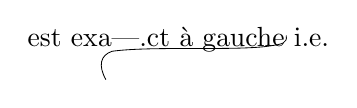
\begin{tikzpicture}[baseline=(b.base),x=1cm,y=1cm]
\node[anchor=base west,inner sep=0pt] (b) at (0,0) {\strut};
\node[anchor=south west,inner sep=0pt] at (-1.0,.22) {\inserted{\handwritten{est ex\unsure{a|.}ct à gauche i.e.}}};
\draw[line width=.3pt] (0,-.12) .. controls (-.10,.06) and (-.07,.19) .. (.08,.24) .. controls (.60,.31) and (1.68,.24) .. (2.10,.31) .. controls (2.23,.33) and (2.31,.34) .. (2.29,.44);
\end{tikzpicture}}commute aux limites projectives finies, on voit donc en particulier que $\mathrm{u}^{\handwritten{*}}$ \uline{est} \deleted{exac} \uline{exact}.
% GRAPHIC G04: typed interlinear insertion, joined to the opening c by a curved leader.
\mbox{
\begin{tikzpicture}[baseline=(b.base),x=1cm,y=1cm]
\node[anchor=base west,inner sep=0pt] (b) at (0,0) {\strut};
\node[anchor=south west,inner sep=0pt] at (-.25,.24) {\inserted{On peut donc dire que}};
\draw[line width=.3pt] (0,-.17) .. controls (-.06,.02) and (-.08,.20) .. (.06,.24) .. controls (1.00,.29) and (3.28,.24) .. (3.48,.31) .. controls (3.54,.33) and (3.55,.38) .. (3.52,.42);
\end{tikzpicture}}\uline{\deleted{C}\handwritten{c}'est \deleted{donc} le foncteur image inverse}
% GRAPHIC G05: the star is definite; a separate small point lies below its right ray.
$\mathrm{u}^{\handwritten{*\!\unsure{\begin{tikzpicture}[baseline=.5ex,x=1ex,y=1ex]\fill (0,0) circle (.05);\end{tikzpicture}}}}$ \deleted{qui}, dans le couple $(\mathrm{u}_{\handwritten{*}},\mathrm{u}^{\handwritten{*}})$, \uline{qui possède les propriétés d'exactitude les plus remarquables}, \deleted{assurant} Ces propriétés assurent que pour toute espèce de structure algébrique
% GRAPHIC G06: Sigma, its insertion leader, and a distinct faint arc under its lower arm.
\mbox{\begin{tikzpicture}[baseline=(b.base),x=1cm,y=1cm]
\node[anchor=base west,inner sep=0pt] (b) at (0,0) {\strut};
\node[anchor=south west,inner sep=0pt] at (.10,.24) {\inserted{\handwritten{$\Sigma$}}};
\draw[line width=.3pt] (0,-.15) .. controls (-.08,.06) and (.04,.17) .. (.24,.21) .. controls (.43,.24) and (.78,.28) .. (1.02,.35) .. controls (1.09,.38) and (1.12,.42) .. (1.10,.46);
\node[anchor=west,inner sep=0pt] at (.18,.23) {\handwritten{\unsure{\begin{tikzpicture}[x=1cm,y=1cm]\draw[line width=.2pt] (0,0) .. controls (.10,-.08) and (.18,-.06) .. (.28,-.02);\end{tikzpicture}}}};
\end{tikzpicture}}\deleted{qui\mbox{
\begin{tikzpicture}[baseline=(x.base)]\node[inner sep=0pt] (x) {\texttt{x}};\end{tikzpicture}}peut} dont les données peuvent se décrire en termes de données de flèches entre les ensembles de base et des ensembles déduits de ceux-ci par application répétée d'opérations de limites projectives finies et de limites inductives quelconques,
% GRAPHIC G07: et pour with the curved leader before tout.
\mbox{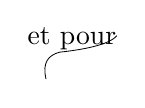
\begin{tikzpicture}[baseline=(b.base),x=1cm,y=1cm]
\node[anchor=base west,inner sep=0pt] (b) at (0,0) {\strut};
\node[anchor=south west,inner sep=0pt] at (-.24,.24) {\inserted{\handwritten{et pour}}};
\draw[line width=.3pt] (0,-.12) .. controls (-.05,.09) and (.03,.18) .. (.17,.22) .. controls (.45,.25) and (.80,.31) .. (.90,.43);
\end{tikzpicture}}tout \handwritten{``}objet de $\underline{\mathrm{E}}'$ muni d'une structure d'espèce $\handwritten{\Sigma}$'' (notion qui a un sens grâce aux propriétés d'exactitude \deleted{de} internes du topos
% GRAPHIC G08: definite E with an additional broad lower retouch; its identity is not decided as a second E.
$\mbox{\begin{tikzpicture}[baseline=(e.base),x=1ex,y=1ex]
\node[inner sep=0pt] (e) at (0,0) {$\mathrm E$};
\node[anchor=center,inner sep=0pt] at (0,-.18) {\unsure{\begin{tikzpicture}[x=1ex,y=1ex]\draw[line width=1.5pt] (-.40,-.12) .. controls (-.23,.12) and (.03,-.10) .. (.20,-.07) .. controls (.40,-.10) and (.30,.25) .. (.24,.30);\end{tikzpicture}}};
\end{tikzpicture}}'$ (II 4.1)), son image \deleted{inverse} par $\mathrm{u}^{\handwritten{*}}$ est muni des mêmes structures. Plutôt que d'entrer dans la tâche peu engageante de donner un sens précis à cet énoncé et de le justifier de façon formelle, nous conseillons au lecteur de
% GRAPHIC G09: typed insertion and its curved leader before se.
\mbox{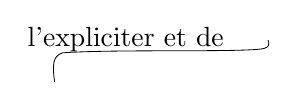
\begin{tikzpicture}[baseline=(b.base),x=1cm,y=1cm]
\node[anchor=base west,inner sep=0pt] (b) at (0,0) {\strut};
\node[anchor=south west,inner sep=0pt] at (-.35,.24) {\inserted{l'expliciter et de}};
\draw[line width=.3pt] (0,-.13) .. controls (-.03,.07) and (-.03,.20) .. (.10,.24) .. controls (.81,.29) and (2.55,.24) .. (2.67,.30) .. controls (2.72,.31) and (2.73,.36) .. (2.71,.40);
\end{tikzpicture}}se convaincre de sa validité pour
% GRAPHIC G10: three detached points descend to the left below the gap after pour; no punctuation function is assigned.
\makebox[0pt][l]{\handwritten{\unsure{\begin{tikzpicture}[baseline=0pt,x=1mm,y=1mm]\fill (1.8,-1.5) ellipse (.16 and .20);\fill (1.1,-2.5) ellipse (.18 and .18);\fill (.4,-3.5) circle (.13);\end{tikzpicture}}}}des espèces de structure telles que celle de groupe, d'anneau, de module sur un anneau, de comodule \deleted{ou\mbox{
\begin{tikzpicture}[baseline=(x.base)]\node[inner sep=0pt] (x) {\texttt{x}};\end{tikzpicture}}de\mbox{
\begin{tikzpicture}[baseline=(x.base)]\node[inner sep=0pt] (x) {\texttt{x}};\end{tikzpicture}}bimodule} sur un anneau, de bigèbre sur un anneau, de torseur sous un groupe. (Dans ces exemples, les trois premières espèces de structure se définis}
% The three typed x impressions in otherwise blank cells are cancellation marks: after qui, ou, and de.
% The last word is cut at the right image edge after the visible fragment ``définis''; no unseen ending is supplied.

\margin{\handwritten{\deleted{(I \unsure{2.11|4.11|4.1})}.}}

% GRAPHIC G11: one long, slightly wavy separator above the footnote.
\handwritten{\figure{
\begin{tikzpicture}[x=1cm,y=1cm]
\draw[line width=.4pt] (0,.03) .. controls (.8,-.08) and (1.0,-.05) .. (1.6,0) .. controls (4.8,.12) and (9.7,-.08) .. (13.0,.04) .. controls (13.5,.06) and (13.9,.10) .. (14.2,.03);
\end{tikzpicture}}}

\deleted{($\handwritten{*}$) \deleted{On p\unsure{eu}t} \deleted{d}\handwritten{D}'ailleurs
% GRAPHIC G12: the raised reference and the three visible stretches of its light leader.
\mbox{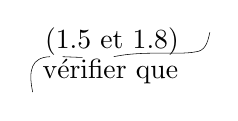
\begin{tikzpicture}[baseline=(b.base),x=1cm,y=1cm]
\node[anchor=base west,inner sep=0pt] (b) at (0,0) {\deleted{vérifier que}};
\node[anchor=south west,inner sep=0pt] at (.03,.29) {\inserted{\handwritten{(1.5 et 1.8)}}};
\draw[line width=.2pt] (-.12,-.17) .. controls (-.18,.12) and (-.13,.27) .. (.10,.28);
\draw[line width=.2pt] (.26,.28) -- (.51,.27);
\draw[line width=.2pt] (.91,.28) .. controls (1.28,.36) and (1.73,.30) .. (1.94,.34) .. controls (2.07,.35) and (2.10,.45) .. (2.13,.59);
\end{tikzpicture}},pour un foncteur $\mathrm{u}_{\handwritten{*}}:\mathrm{E}\handwritten{\longrightarrow}\mathrm{E}'$ resp. $\mathrm{u}^{\handwritten{*}}:\mathrm{E}'\handwritten{\longrightarrow}\mathrm{E}$ donné, \deleted{d}\handwritten{\unsure{c|d}}e foncteur admet un adjoint à gauche (resp. à droite si et seulement si il commute aux
% GRAPHIC G13: typed underlined U and hyphen, with a pen leader before limites.
\mbox{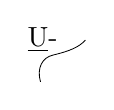
\begin{tikzpicture}[baseline=(b.base),x=1cm,y=1cm]
\node[anchor=base west,inner sep=0pt] (b) at (0,0) {\strut};
\node[anchor=south west,inner sep=0pt] at (-.17,.24) {\inserted{$\underline{\mathrm U}$-}};
\draw[line width=.3pt] (0,-.13) .. controls (-.05,.04) and (.02,.18) .. (.16,.21) .. controls (.37,.26) and (.49,.31) .. (.57,.40);
\end{tikzpicture}}limites projectives (resp. aux $\underline{\mathrm{U}}$-limites inductives). \deleted{\unsure{D'ailleurs}
% GRAPHIC G14: a separate light diagonal tail below the end of the cancelled word.
\makebox[0pt][l]{\unsure{\begin{tikzpicture}[baseline=0pt,x=1cm,y=1cm]\draw[line width=.2pt] (-.14,-.07) .. controls (-.02,-.12) and (.10,-.24) .. (.24,-.26);\end{tikzpicture}}}, c'est une conséquence immédiate de 1.2.
% GRAPHIC G15: cancelled subdivision with an upper light trace and a separate lower heavy overrun.
\mbox{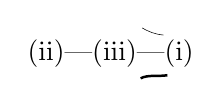
\begin{tikzpicture}[baseline=(s.base),x=1cm,y=1cm]
\node[inner sep=0pt] (s) at (0,0) {\unsure{(ii)|(iii)|(i)}};
\draw[line width=.2pt] (.40,.33) .. controls (.49,.28) and (.56,.25) .. (.67,.24);
\draw[line width=.9pt] (.38,-.31) .. controls (.47,-.26) and (.61,-.29) .. (.72,-.27);
\end{tikzpicture}}}}
% The right edge after ``droite'' is cropped; no unseen closing parenthesis has been added.
